\chapter{Separation by Unknown Modulation}

\marginpar{This chapter is based on the work that has been published at the ICASSP conference in 2016. The work has been done in close collaboration with Antoine Liutkus from INRIA, France and Roland Badeu from ParisTech France.}


% Add introduction to matrix factorization based things

The first set of approaches we consider is the identification of redundancy in the accompaniment through the assumption that its spectrogram may be well represented by only a few components. Techniques exploiting this idea then focus on algebraic methods that decompose the mixture spectrogram into the product of a few template spectra activated over time. One way to do so is via non-negative matrix factorization (NMF) \cite{lee99,lee01}, which incorporates non-negative constraints. In Figure~\ref{fig:methods_low_rank}, we picture methods exploiting such techniques. After factorization, we obtain several spectra, along with their activations over time. A subsequent step is the clustering of these spectra (and activations) into the lead or the accompaniment. Separation is finally performed by deriving Wiener filters to estimate the lead and the accompaniment from the mixture. For related applications of NMF in music analysis, the reader is referred to \cite{smaragdis03,virtanen07,fevotte09}.

Vembu and Baumann proposed to use NMF (and also ICA \cite{common94}) to separate vocals from mixtures \cite{vembu05}. They first discriminated between vocal and non-vocal sections in a mixture by using different combinations of features, such as MFCCs \cite{david80}, perceptual linear predictive (PLP) coefficients \cite{hermansky90}, and log frequency power coefficients (LFPC) \cite{nwe04}, and training two classifiers, namely neural networks and support vector machines (SVM). They then applied redundancy reduction techniques on the TF representation of the mixture to separate the sources \cite{casey00}, by using NMF (or ICA). The components were then grouped as vocal and non-vocal by reusing a vocal/non-vocal classifier with MFCC, LFPC, and PLP coefficients.

Chanrungutai and Ratanamahatana proposed to use NMF with automatic component selection\cite{chanrungutai08,chanrungutai082}. They first decomposed the mixture spectrogram using NMF with a fixed number of basis components. They then removed the components with brief rhythmic and long-lasting continuous events, assuming that they correspond to instrumental sounds. They finally used the remaining components to reconstruct the singing voice, after refining them using a high-pass filter.

Marxer and Janer proposed an approach based on a Tikhonov regularization~\cite{tikhonov63} as an alternative to NMF, for singing voice separation~\cite{marxer122}. Their method sacrificed the non-negativity constraints of the NMF in exchange for a computationally less expensive solution for spectrum decomposition, making it more interesting in low-latency scenarios.

Yang et al. proposed a Bayesian NMF approach \cite{yang14,chien15}. Following the approaches in \cite{cemgil09} and \cite{schmidt09}, they used a Poisson distribution for the likelihood function and exponential distributions for the model parameters in the NMF algorithm, and derived a variational Bayesian EM  algorithm \cite{dempster77} to solve the NMF problem. They also adaptively determined the number of bases from the mixture. They finally grouped the bases into singing voice and background music by using a \textit{k}-means clustering algorithm \cite{spiertz09} or an NMF-based clustering algorithm.

In a different manner, Smaragdis and Mysore proposed a user-guided approach for removing sounds from mixtures by humming the target sound to be removed, for example a vocal track \cite{smaragdis09}. They modeled the mixture using probabilistic latent component analysis (PLCA) \cite{smaragdis07}, another equivalent formulation of NMF. One key feature of exploiting user input was to facilitate the grouping of components into vocals and accompaniment, as humming helped to identify some of the parameters for modeling the vocals.

Nakamuray and Kameoka proposed an $L_p$-norm NMF~\cite{nakamuray15}, with $p$ controlling the sparsity of the error. They developed an algorithm for solving this NMF problem based on the auxiliary function principle \cite{ortega70,kameoka06}. Setting an adequate number of bases and $p$ taken as small enough allowed them to estimate the accompaniment as the low-rank decomposition, and the singing voice as the error of the approximation, respectively. Note that, in this case, the singing voice was not explicitly modeled as a sparse component but rather corresponded to the error which happened to be constrained as sparse. The next subsection will actually deal with approaches that explicitly model the vocals as the sparse component.
% end zafar

% \section{Modulation Spectrogram based Separation}

% Intro commonfate START
% Unknown modulation!
Sound source separation continues to be a very active field of research~\cite{vincent14} with a variety of applications. Many recent contributions are based on the popular non-negative matrix factorization (NMF). The way NMF factorizes a spectrogram matrix into frequency and activation templates makes it possible to easily design algorithms in an intuitive way. At the same time, it provides a rank reduction, needed to decompose mixtures into their source components.
In the past, many NMF-based source separation methods have been developed~\cite{smaragdis03, smaragdis04, virtanen07}. Expanding the NMF to tensors allows to incorporate more complex models, useful in many applications like multi-channel separation. Extensions to NMF such as shift-invariance or convolutions were carried over to non-negative tensor (NTF) based algorithms~\cite{fitzgerald05, fitzgerald08, fitzgerald06, fevotte10, ozerov11}. These approaches, relying on decomposing mixtures of musical instruments, work well when certain assumptions hold to be true.
One is that spectral harmonics only partially overlap. However, when two sources share the same fundamental frequency, almost all partials do overlap, making it difficult for NMF-based algorithms to learn unique templates. Another assumption is that all spectral and temporal templates semantically correspond to musical notes, forming a dictionary of musically meaningful atoms.
This does not hold for instruments with time-varying fluctuations. These effects can typically be found in musical instruments like strings and brass, when played with vibrato. In a setting where two musical instruments with vibrato play in unison, both assumptions could break, which makes it a challenging scenario~\cite{stoeter14}.
% Intro commonfate START

When processing such mixtures with a representation based on a standard NMF and the magnitude spectrogram, it is hard to model the sources with only a few spectral templates. Instead of increasing the number of templates per source, Hennequin proposes~\cite{hennequin11} frequency-dependent activation matrices by using a source/filter-based model.
Since the vibrato does not only cause frequency modulation (FM) but also amplitude modulation (AM), so-called modulation spectra can be used to identify the modulation pattern. This is often calculated by taking the Fourier transform of a magnitude spectrum. Thus, the \emph{modulation spectrogram} has already gathered much attention in speech recognition~\cite{greenberg97,kingsbury98} and classification~\cite{kinnunen08, markaki09}.
Barker and Virtanen~\cite{barker13} were the first to propose a modulation tensor representation for single channel source separation. This allows to elegantly apply factorization on the tensor by using the well known PARAFAC/CANDECOMP (CP) decomposition.

In this work we introduce a novel tensor signal representation which additionally exploits similarities in the frequency direction. We can therefore make use of dependencies between modulations of neighbouring bins. This is similar to the recently proposed High-Resolution Nonnegative Matrix Factorization
model that accounts for dependencies in the time-frequency plane (HR-NMF
~\cite{badeau11}). In short, HR-NMF models each complex entry of a time-frequency transform of an audio signal as a linear combination of its neighbours, enabling the modelling of damped sinusoids, along with an independent
innovation. This model was generalized to multichannel mixtures in~\cite{badeau13a,badeau14}
and was shown to provide considerably better oracle performance for source separation than alternative models in~\cite{magron15a}.
Indeed, even though some variational approximations were introduced
in~\cite{badeau13} to strongly reduce their complexity,
those algorithms are often demanding for practical applications.
In this paper, we propose to relax some assumptions of HR-NMF in the interest of simplifying the estimation procedure. The core idea is to divide the complex spectrogram into modulation patches in order to group common modulation in time and frequency direction. We call this the \emph{Common Fate Model} (CFM), borrowing from the Gestalt theory, which describes how human perception merges objects that move together over time. Bregman~\cite{bregman94} described the Common Fate theory for auditory scene analysis as the ability to group sound objects based on their common motion over time, as occurs with frequency modulations of harmonic partials. As outlined by Bregman, the human ability to detect and group sound sources by small differences in FM and AM is outstanding. Also, it turns out that humans are especially sensitive to modulation frequencies around 5~Hz, which is the typical vibrato frequency that many musicians produce naturally.
% Intro commonfate END

%\from dafx
%%%%%%%%%%%%%%%%%%%%%%%%%%%%%%%%%%%%%%%%%%%%%%%%%%%%%%%%%%%%%%%%%%%%%%%%%%%%%%%%%
\section{Separating by Amplitude Modulation}
\label{sub:am}

\begin{figure}[H]
    \centering
    \tiny
    \subfloat[Input]{
       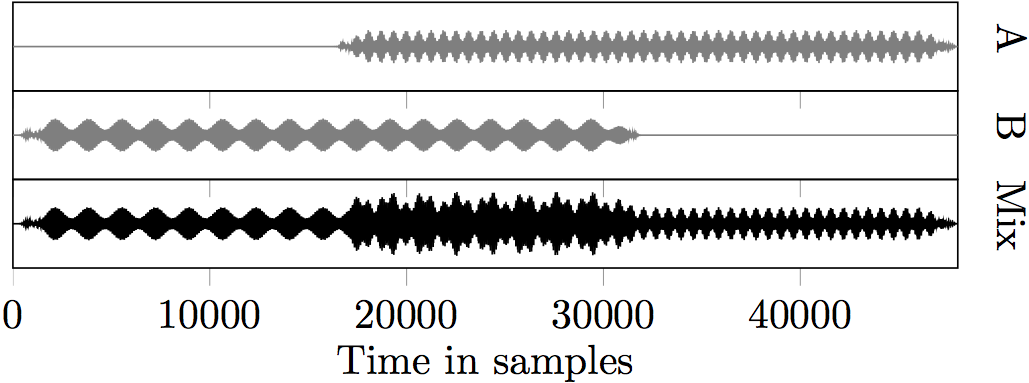
\includegraphics[width=0.92\columnwidth]{Chapters/05_Separation_Known/figures/Timepdf-crop.png}	   		  \hspace{-7mm}
    }\hfill
    \subfloat[Spectrogram]{
       % This file was created by matlab2tikz% This file was created by matlab2tikz v0.4.7 (commit 3442858e5a642c135c5e9dab6a960bee5b9c6f8d) running on MATLAB 8.2.
% Copyright (c) 2008--2014, Nico Schlmer <nico.schloemer@gmail.com>
% All rights reserved.
% Minimal pgfplots version: 1.3
%
% The latest updates can be retrieved from
%   http://www.mathworks.com/matlabcentral/fileexchange/22022-matlab2tikz
% where you can also make suggestions and rate matlab2tikz.
%
\begin{tikzpicture}[font=\small]

\begin{axis}[%
width=0.225\columnwidth,
height=3.5cm,
axis on top,
xminorgrids=true,
minor xtick={1.5,2.5},
scale only axis,
xtick={1,2},
xmin=0.5,
xmax=2.5,
ymin=0.5,
ymax=137.5,
name=plot2,
xlabel=Gain Components,
ylabel=Modulation Frequency Bins,
every axis y label/.style={at={(current axis.north east)},below=18mm,xshift=4mm},
y label style={rotate=-90},
]
\addplot [forget plot] graphics [xmin=0.5,xmax=2.5,ymin=0.5,ymax=137.5] {Chapters/dafx/figures/AMPlots/GAS-1_scaled.png};
\end{axis}

\begin{axis}[%
width=0.225\columnwidth,
height=3.5cm,
xminorgrids=true,
minor xtick={1.5,2.5},
axis on top,
scale only axis,
xtick={1,2},
xmin=0.5,
xmax=2.5,
ymin=0.5,
ymax=145.5,
xlabel=Basis Components,
ylabel=Frequency Bins,
every axis y label/.style={at={(current axis.north east)},below=18mm,xshift=4mm},
y label style={rotate=-90},
at=(plot2.left of south west),
anchor=right of south east
]
\addplot [forget plot] graphics [xmin=0.5,xmax=2.5,ymin=0.5,ymax=145.5] {Chapters/dafx/figures/AMPlots/GAS-2_scaled.png};
\end{axis}

\begin{axis}[%
width=0.225\columnwidth,
height=3.5cm,
xminorgrids=true,
minor xtick={1.5,2.5},
axis on top,
scale only axis,
xtick={1,2},
xmin=0.5,
xmax=2.5,
ymin=0.5,
ymax=81.5,
xlabel=Activation Components,
ylabel=Frames,
every axis y label/.style={at={(current axis.north east)},below=18mm,xshift=4mm},
y label style={rotate=-90},
at=(plot2.right of south east),
anchor=left of south west
]
\addplot [forget plot] graphics [xmin=0.5,xmax=2.5,ymin=0.5,ymax=81.5] {Chapters/dafx/figures/AMPlots/GAS-3_scaled.png};
\end{axis}
\end{tikzpicture}%
 v0.4.7 (commit 3442858e5a642c135c5e9dab6a960bee5b9c6f8d) running on MATLAB 8.2.
% Copyright (c) 2008--2014, Nico Schlmer <nico.schloemer@gmail.com>
% All rights reserved.
% Minimal pgfplots version: 1.3
%
% The latest updates can be retrieved from
%   http://www.mathworks.com/matlabcentral/fileexchange/22022-matlab2tikz
% where you can also make suggestions and rate matlab2tikz.
%
\begin{tikzpicture}[font=\small]

\begin{axis}[%
    /pgf/number format/.cd,
           use comma,
           1000 sep={},
width=0.35\columnwidth,
height=3.5cm,
axis on top,
scale only axis,
xmin=0.5,
xmax=1497.5,
ymin=0.5,
ymax=145.5,
xlabel=Frames,
ylabel=Frequency Bins,
every axis y label/.style={at={(current axis.north east)},below=18mm,xshift=4mm},
y label style={rotate=-90},
]
\addplot [forget plot] graphics [xmin=0.5,xmax=1497.5,ymin=0.5,ymax=145.5] {Chapters/05_Separation_Known/figures/AMPlots/STFT-1_scaled.png};
\end{axis}
\end{tikzpicture}%
%
    }%
    \subfloat[Tensor Slice]{
       % This file was created by matlab2tikz v0.4.7 (commit 3442858e5a642c135c5e9dab6a960bee5b9c6f8d) running on MATLAB 8.2.
% Copyright (c) 2008--2014, Nico Schlmer <nico.schloemer@gmail.com>
% All rights reserved.
% Minimal pgfplots version: 1.3
%
% The latest updates can be retrieved from
%   http://www.mathworks.com/matlabcentral/fileexchange/22022-matlab2tikz
% where you can also make suggestions and rate matlab2tikz.
%
\begin{tikzpicture}[font=\small]

\begin{axis}[%
width=0.73\textwidth,
height=3.5cm,
axis on top,
trim axis left,
scale only axis,
xmin=0.5,
xmax=81.5,
ymin=0.5,
ymax=137.5,
xlabel=Frames,
ylabel=Modulation Frequency Bins,
every axis y label/.style={at={(current axis.north east)},below=18mm,xshift=8mm},
y label style={rotate=-90},
]
\addplot [forget plot] graphics [xmin=0.5,xmax=81.5,ymin=0.5,ymax=137.5] {Chapters/05_Separation_Known/figures/AMPlots/Tmod-1_scaled.png};
\end{axis}
\end{tikzpicture}%
%
    }\hfill

    \subfloat[NMF]{
     	% This file was created by matlab2tikz v0.4.7 (commit 3442858e5a642c135c5e9dab6a960bee5b9c6f8d) running on MATLAB 8.2.
% Copyright (c) 2008--2014, Nico Schlmer <nico.schloemer@gmail.com>
% All rights reserved.
% Minimal pgfplots version: 1.3
%
% The latest updates can be retrieved from
%   http://www.mathworks.com/matlabcentral/fileexchange/22022-matlab2tikz
% where you can also make suggestions and rate matlab2tikz.
%
\begin{tikzpicture}[font=\small]

\begin{axis}[%
/pgf/number format/.cd, use comma, 1000 sep={},
width=0.225\columnwidth,
height=3.5cm,
axis on top,
scale only axis,
xtick={1,2},
xminorgrids=true,
minor xtick={1.5},
xmin=0.5,
xmax=2.5,
ymin=0.5,
ymax=145.5,
name=plot1,
xlabel=Basis Components,
ylabel=Frequency Bins,
every axis y label/.style={at={(current axis.north east)},below=18mm,xshift=8mm},
y label style={rotate=-90},
]
\addplot [forget plot] graphics [xmin=0.5,xmax=2.5,ymin=0.5,ymax=145.5] {Chapters/05_Separation_Known/figures/AMPlots/WH-1_scaled.png};
\end{axis}

\begin{axis}[%
/pgf/number format/.cd, use comma, 1000 sep={},
width=0.225\columnwidth,
height=3.5cm,
axis on top,
scale only axis,
xminorgrids=true,
minor xtick={1.5},
xtick={1,2},
xmin=0.5,
xmax=2.5,
ymin=0.5,
ymax=1497.5,
xlabel=Activation Components,
ylabel=Frames,
every axis y label/.style={at={(current axis.north east)},below=18mm,xshift=8mm},
y label style={rotate=-90},
at=(plot1.right of south east),
anchor=left of south west
]
\addplot [forget plot] graphics [xmin=0.5,xmax=2.5,ymin=0.5,ymax=1497.5] {Chapters/05_Separation_Known/figures/AMPlots/WH-2_scaled.png};
\end{axis}
\end{tikzpicture}%
%
    }\hfill
    \subfloat[Non-Negative Tensor Factorization]{
       % This file was created by matlab2tikz v0.4.7 (commit 3442858e5a642c135c5e9dab6a960bee5b9c6f8d) running on MATLAB 8.2.
% Copyright (c) 2008--2014, Nico Schlmer <nico.schloemer@gmail.com>
% All rights reserved.
% Minimal pgfplots version: 1.3
%
% The latest updates can be retrieved from
%   http://www.mathworks.com/matlabcentral/fileexchange/22022-matlab2tikz
% where you can also make suggestions and rate matlab2tikz.
%
\begin{tikzpicture}[font=\small]

\begin{axis}[%
width=0.15\columnwidth,
height=3.5cm,
axis on top,
xminorgrids=true,
minor xtick={1.5,2.5},
scale only axis,
xtick={1,2},
xmin=0.5,
xmax=2.5,
ymin=0.5,
ymax=137.5,
name=plot2,
xlabel=Gain Components,
ylabel=Modulation Frequency Bins,
every axis y label/.style={at={(current axis.north east)},below=18mm,xshift=8mm},
y label style={rotate=-90},
]
\addplot [forget plot] graphics [xmin=0.5,xmax=2.5,ymin=0.5,ymax=137.5] {Chapters/05_Separation_Known/figures/AMPlots/GAS-1_scaled.png};
\end{axis}

\begin{axis}[%
width=0.15\columnwidth,
height=3.5cm,
xminorgrids=true,
minor xtick={1.5,2.5},
axis on top,
scale only axis,
xtick={1,2},
xmin=0.5,
xmax=2.5,
ymin=0.5,
ymax=145.5,
xlabel=Basis Components,
ylabel=Frequency Bins,
every axis y label/.style={at={(current axis.north east)},below=18mm,xshift=8mm},
y label style={rotate=-90},
at=(plot2.left of south west),
anchor=right of south east
]
\addplot [forget plot] graphics [xmin=0.5,xmax=2.5,ymin=0.5,ymax=145.5] {Chapters/05_Separation_Known/figures/AMPlots/GAS-2_scaled.png};
\end{axis}

\begin{axis}[%
width=0.15\columnwidth,
height=3.5cm,
xminorgrids=true,
minor xtick={1.5,2.5},
axis on top,
scale only axis,
xtick={1,2},
xmin=0.5,
xmax=2.5,
ymin=0.5,
ymax=81.5,
xlabel=Activation Components,
ylabel=Frames,
every axis y label/.style={at={(current axis.north east)},below=18mm,xshift=8mm},
y label style={rotate=-90},
at=(plot2.right of south east),
anchor=left of south west
]
\addplot [forget plot] graphics [xmin=0.5,xmax=2.5,ymin=0.5,ymax=81.5] {Chapters/05_Separation_Known/figures/AMPlots/GAS-3_scaled.png};
\end{axis}
\end{tikzpicture}%
%
    }\hfill
    \caption{Example of separating a mixture of two amplitude modulated signals by NMF and Modulation-NTF. \\ \textbf{(a)} Mixture of two sinusoids at $440$ Hz with AM of $4.7$ Hz and $12.6$ Hz (fs=$8$ kHz), \textbf{(b)} STFT (FFT length = 256), \textbf{(c)} Slice of Modulation Tensor (FFT length = 256),  \textbf{(d)} $\mathbf{W} \times \mathbf{H}$ Result of Non-Negative Matrix Factorization ($\beta = 1$) after 100 iterations, \textbf{(e)}  $\mathbf{G} \times \mathbf{A} \times \mathbf{S} $ Result of Non-Negative Tensor Factorization ($\beta = 1$) after 100 iterations,}
    \label{fig:tensor}
\end{figure}

Amplitude modulation is normally not present, isolated in acoustical instruments. However electric pianos like Rhodes or Wurlitzers can generate a tremolo effect. Using the amplitude modulation to separate mixtures has already been done in \cite{li09} which makes use of the concept of \emph{Common Amplitude Modulation}.

\textsc{CAM} is effectively the property of harmonics that share the same amplitude modulation across the bins.
One way of analyzing it is a modulation spectrogram which is a frequency-frequency representation of a time domain input signal.
There are also other ways to generate a modulation spectrum.
A complete signal representation can be archived by a modulation tensor which holds the modulation spectrograms for each time frame.

% TODO add more info about how to form a modulation tensor for AM.
% the key point is that after the TF transform the magnitude has to be taken to compute the amplitude modulation. Computing the frequency modulation spectrogram is not possble in a simple way. WHY?

% Known modulation
Barker and Virtanen \cite{barker13} found a way to utilize the modulation tensor for single channel source separation. Standard NMF models the spectrogram by the sum of $K$ components which are each factored into frequency/basis and time/activations components:
\begin{equation}
   \mathbf{X}_{n,m} \approx \sum_{k=1}^{K}\mathbf{W_{n,k}}\times \mathbf{H_{k,m}}.
\end{equation}
Non-negative Tensor factorization approximates a modulation tensor by a product of three matrices containing the frequency/basis, time/activation signals, and the modulation gain for each component. Compared to \cite{barker13} we choose to generate the modulation tensor in way that is simpler and easier to invert. Barker and Virtanen use a Gammatone filter bank and  rectification to model the characteristics of the human auditory system. We used a two-stage DFT filter bank where the modulation domain is based on  magnitude spectrograms. Although this can give perceptually less optimal results, each step can be directly inverted by using the complex representation. Barker already showed that the NTF based approach gives better results on speech signals. We found that this approach can be used to separate two instrument mixtures by their amplitude modulation characteristics and is therefore ideal for the unison scenario.

In Figure~\ref{fig:sk_tensor} we show the factorization of a simple amplitude modulated input signal for comparison. The signal consists of two sinusoids which are linearly mixed. Both share the same carrier frequency but have different amplitude modulation frequencies. We choose a factorization into $K=2$ components. From the activation components one can see that NMF is not able to separate the two signals sufficiently. NTF gives a smoother activation matrix and is able to generate the output with the separated amplitude modulations on each sinusoid. The modulation frequency gain matrix shows the two modulation frequency templates and the DC-component.

\begin{figure}[H]
\begin{center}
\begin{tabular}{c}
	\\
   Spectrogram of two sinusoids with same carrier\\
   frequency but different amplitude modulation frequency.\\[6pt]
	 \\
    Spectrogram of two sinusoids with same carrier\\
    frequency but different amplitude modulation frequency.\\[6pt]
	% This file was created by matlab2tikz v0.4.7 (commit 3442858e5a642c135c5e9dab6a960bee5b9c6f8d) running on MATLAB 8.2.
% Copyright (c) 2008--2014, Nico Schlmer <nico.schloemer@gmail.com>
% All rights reserved.
% Minimal pgfplots version: 1.3
%
% The latest updates can be retrieved from
%   http://www.mathworks.com/matlabcentral/fileexchange/22022-matlab2tikz
% where you can also make suggestions and rate matlab2tikz.
%
\begin{tikzpicture}[font=\small]

\begin{axis}[%
/pgf/number format/.cd, use comma, 1000 sep={},
width=0.225\columnwidth,
height=3.5cm,
axis on top,
scale only axis,
xtick={1,2},
xminorgrids=true,
minor xtick={1.5},
xmin=0.5,
xmax=2.5,
ymin=0.5,
ymax=145.5,
name=plot1,
xlabel=Basis Components,
ylabel=Frequency Bins,
every axis y label/.style={at={(current axis.north east)},below=18mm,xshift=8mm},
y label style={rotate=-90},
]
\addplot [forget plot] graphics [xmin=0.5,xmax=2.5,ymin=0.5,ymax=145.5] {Chapters/05_Separation_Known/figures/AMPlots/WH-1_scaled.png};
\end{axis}

\begin{axis}[%
/pgf/number format/.cd, use comma, 1000 sep={},
width=0.225\columnwidth,
height=3.5cm,
axis on top,
scale only axis,
xminorgrids=true,
minor xtick={1.5},
xtick={1,2},
xmin=0.5,
xmax=2.5,
ymin=0.5,
ymax=1497.5,
xlabel=Activation Components,
ylabel=Frames,
every axis y label/.style={at={(current axis.north east)},below=18mm,xshift=8mm},
y label style={rotate=-90},
at=(plot1.right of south east),
anchor=left of south west
]
\addplot [forget plot] graphics [xmin=0.5,xmax=2.5,ymin=0.5,ymax=1497.5] {Chapters/05_Separation_Known/figures/AMPlots/WH-2_scaled.png};
\end{axis}
\end{tikzpicture}%
 \\
    Non-Negative Matrix Factorization \\[6pt]
	 \\
    Non-Negative Tensor Factorization\\[6pt]
\end{tabular}
\caption{Example of processing a non-stationary amplitude modulated signal with NMF and Modulation-NTF}
\label{fig:sk_tensor}
\end{center}
\end{figure}

\begin{figure}[H]
\begin{center}
\begin{tikzpicture}[block/.style={draw, minimum width=40pt, outer sep=0pt}]
  % small STFTs
  \node(A)[block, minimum height=30pt]             {STFT};
  \node(B)[block, below=of A, minimum height=30pt] {STFT};

   % huge STFT
  \node(STFT)[block, fit=(A)(B),left=of A.north west,anchor=north east, inner sep=0] {STFT};

  % arrow for input signal x
  \draw[-latex] ($(STFT.west) - (1, 0)$) |- (STFT.west) node [pos=0.75, above] (TextNode) {$x(n)$};

  % arrows to connect huge STFT with small STFTs plus labeling
  \draw[-latex] (STFT.east) |- (A.west) node [pos=0.75, above, font=\small] (TextNode) {$|x_c(n)|$};
  \draw[-latex] (STFT.east) |- (B.west) node [pos=0.75, above, font=\small] (TextNode) {$|x_c(n)|$};

  % arrows from node A to right side
  \draw[-latex] ($(A.east) + (0,0.3)$) -- ($(A.east) + (1,0.3)$);
  \draw[-latex] ($(A.east)$) -- ($(A.east) + (1,0)$);
  \draw[-latex] ($(A.east) + (0,-0.3)$) -- ($(A.east) + (1,-0.3)$);

  % arrows from node B to right side
  \draw[-latex] ($(B.east) + (0,0.3)$) -- ($(B.east) + (1,0.3)$);
  \draw[-latex] ($(B.east)$) -- ($(B.east) + (1,0)$);
  \draw[-latex] ($(B.east) + (0,-0.3)$) -- ($(B.east) + (1,-0.3)$);


  % dotted lines between small STFTs
  \draw[dotted] ($(A.south) + (0, -0.3)$) |- ($(B.north) + (0, 0.3)$);
\end{tikzpicture}
\caption{Demonstration of signal separation based on NTF}
\label{fig:sk_ntfdemo}
\end{center}
\end{figure}


\section{Chapter Conclusion and Outlook}

While methods focusing on harmonic models for the lead often fall short in their expressive power for the accompaniment, the methods we reviewed in this section are often observed to suffer exactly from the converse weakness, namely they do not provide an adequate model for the lead signal. Hence, the separated vocals often will feature interference from unpredictable parts from the accompaniment, such as some percussion or effects which occur infrequently.

Furthermore, even if the musical accompaniment will exhibit more redundancy, the vocals part will also be redundant to some extent, which is poorly handled by these methods. When the lead signal is not vocals but played by some lead instrument, its redundancy is even more pronounced, because the notes it plays lie in a reduced set of fundamental frequencies. Consequently, such methods would include the redundant parts of the lead within the accompaniment estimate, for example, a steady humming by a vocalist.
